\documentclass[25pt, a0paper, portrait, margin=0mm, innermargin=0pt, blockverticalspace=0mm, colspace=0mm, subcolspace=0mm, roundedcorners=0]{tikzposter} %Default values for poster format options.
\tikzposterlatexaffectionproofoff% remove tikzposter logo

\pdfinfo{
   /Author (Maurice Frank)
   /Title  (Problems using deep generative models for probabilistic audio source separation)
}


\usepackage{newpxtext}
\usepackage{amsmath}
\usepackage{amssymb}
\usepackage[sc]{mathpazo}
\usepackage{dsfont}
\usepackage{nicefrac}
\usepackage{bm}
\usepackage[binary-units]{siunitx}
\usepackage{mathtools}
\usepackage{bigints}
\usepackage{tikz}
\usetikzlibrary{
    3d,
    arrows,
    arrows.meta,
    backgrounds,
    bending,
    calc,
    chains,
    decorations.pathmorphing,
    decorations.pathreplacing,
    graphs,
    matrix,
    patterns,
    positioning,
    quotes,
    shapes.arrows,
    shapes.geometric,
    shapes.misc,
}
\usepackage{pgfplots}
\usepgfplotslibrary{
    groupplots,
    dateplot,
}
\pgfplotsset{compat=newest}
\makeatletter
\pgfset{
  /pgf/decoration/randomness/.initial=2,
  /pgf/decoration/wavelength/.initial=100
}
\pgfdeclaredecoration{sketch}{init}{
  \state{init}[width=0pt,next state=draw,persistent precomputation={
    \pgfmathsetmacro\pgf@lib@dec@sketch@t0
  }]{}
  \state{draw}[width=\pgfdecorationsegmentlength,
  auto corner on length=\pgfdecorationsegmentlength,
  persistent precomputation={
    \pgfmathsetmacro\pgf@lib@dec@sketch@t{mod(\pgf@lib@dec@sketch@t+pow(\pgfkeysvalueof{/pgf/decoration/randomness},rand),\pgfkeysvalueof{/pgf/decoration/wavelength})}
  }]{
    \pgfmathparse{sin(2*\pgf@lib@dec@sketch@t*pi/\pgfkeysvalueof{/pgf/decoration/wavelength} r)}
    \pgfpathlineto{\pgfqpoint{\pgfdecorationsegmentlength}{\pgfmathresult\pgfdecorationsegmentamplitude}}
  }
  \state{final}{}
}
\tikzset{xkcd/.style={line width=1.5mm,decorate,decoration={sketch,segment length=1pt,amplitude=1pt}}}
\makeatother
\tikzstyle{arrow}=[-{Latex[length=15mm, width=4mm]}]
\tikzset{every picture/.style={line width=1.5mm}}
\tikzstyle{bigarrow}=[-{Latex[length=30mm, width=8mm]}, line width=4mm]

\graphicspath{{graphics/}} % set of paths to search for images
\usepackage[export]{adjustbox}
\usepackage[many]{tcolorbox}
\usepackage[labelfont=bf]{caption}
\usepackage{subfigure}

\newcommand*{\B}[1]{\ifmmode\bm{#1}\else\textbf{#1}\fi}
\newcommand*{\I}[1]{\ifmmode\mathit{#1}\else\textit{#1}\fi}
\renewcommand*{\t}[1]{\ifmmode\text{#1}\else #1 \fi}
\newcommand\D{\ensuremath{\mathcal{D}}}
\newcommand\m{\ensuremath{\B{m}}}
\newcommand\s{\ensuremath{\B{s}}}
\newcommand\z{\ensuremath{\B{z}}}
\newcommand\x{\ensuremath{\B{x}}}
\newcommand{\aprxpost}{{q_{\B{\pi}_k}(\s_k|\m)}}

\definecolor{green}{rgb}	{0.6, 0.59, 0.1}
\definecolor{yellow}{rgb}	{0.84, 0.6, 0.13}
\definecolor{red}{rgb}	{0.8, 0.14, 0.11}
\definecolor{orange}{rgb}	{0.84, 0.36, 0.05}
\definecolor{blue}{rgb}	{0.27, 0.52, 0.53}
\definecolor{purple}{rgb}	{0.69, 0.38, 0.53}
\definecolor{aqua}{rgb}	{0.41, 0.62, 0.42}
\definecolor{extlinkcolor}{rgb}	{0.03, 0.4, 0.47}
\definecolor{intlinkcolor}{rgb}	{0.69, 0.23, 0.01}

\definecolor{primary}{HTML}{524667}
\newcommand\NameBlock[1]{\node[fit=(blockbody)(blocktitle),inner sep=-5pt] (#1) {};}
\usetheme{Simple}

\begin{document}
    \useblockstyle{Basic}

    \maketitle[titletotopverticalspace=0cm, width=\linewidth, roundedcorners=0, linewidth=0pt,titletoblockverticalspace=0cm]

    \makeatletter
        \setlength{\TP@blocktop}{.5\textheight}
    \makeatother

    \colorlet{blockbodybgcolor}{white}
    \block[linewidth=0pt, roundedcorners=0]{}{
        \parbox{\linewidth}{\centering \bfseries \huge \color{primary} Problems using deep generative models for probabilistic audio source separation}
        \parbox{\linewidth}{\tiny ~~\\}
        \parbox{\linewidth}{\centering \color{primary} \Large
            \begin{tikzpicture}[scale=1, every node/.style={scale=0.9}]
                \node[circle,draw,inner sep=1.5cm,fill overzoom image=frank] (frank) {};
                \node[right=0.7cm of frank,align=left] (franktext) {Maurice Frank\\maurice.frank@posteo.de};
                \node[right=20cm of frank,circle,draw,inner sep=1.5cm,fill overzoom image=ilse] (ilse) {};
                \node[right=0.7cm of ilse,align=left] (ilsetext) {Maximilian Ilse\\m.ilse@uva.nl};
                \node [anchor=west,fill=primary,text width=14cm,text=white,scale=0.6,rotate=-15] (note) at (11,2.2) {Searching for PhD in these topics!};
                \draw [arrow, primary] (note.west) to[out=-15, in=50] (frank.north east);
            \end{tikzpicture}
        }
    }

    \block[linewidth=0pt, roundedcorners=0]{}{
        \centering
        \begin{minipage}{.5\textwidth}
            \B{Idea}: Train generative prior models for different sources of musical sounds. Use those probability density functions to solve multi-instrument tasks like audio source separation. For example we can pose source separation as the sampling procedure of finding the set of fitting samples from each distribution. This could be achieved with Langevin dynamics, but \dots
        \end{minipage}
    }

    \block{}{
        \vspace{-1em}
        \centering
        {\LARGE \textbf{What happens if we train a generative model for sound sources separately?}}\\%
        \begin{tikzpicture}[thick,scale=1.5, every node/.style={transform shape}]
            \foreach \source/\offset in {other/0,drums/1,vocals/2,bass/3}{%
            \begin{scope}
                \node    (stem) at (13*\offset, 0)   {\includegraphics[width=80pt]{../data/images/\source.png}};
                \node[right=20pt of stem,draw] (flow)   {\(p(\s_{\source})\)};
                \node[right=15pt of flow]      (prior)  {\includegraphics[width=85pt]{dist/\source}};
                \draw[arrow] ([xshift=-1cm]stem.east) -- (flow);
                \draw[arrow] (flow) -- ([xshift=1cm]prior.west);
            \end{scope}}%

            \draw[xkcd] (24.5,-2) .. controls (24.5, -4) and (37.5, -4) .. (37.5,-7);
            \draw[xkcd] (24.5,-2) .. controls (24.5, -4) and (11.5, -4) .. (11.5,-7);
            \node[align=center] (label) at (24.5, -6) {Two types of model\\each trained on real instruments and toy data};
        \end{tikzpicture} 
        
        \vspace*{50pt}

        \begin{minipage}{0.9\linewidth}
            \begin{minipage}{.5\textwidth}
                \centering
                {\Large \textbf{FloWaveNet} (normalizing flow)}\\%
                \vspace*{0.5cm}
                \begin{tikzfigure}
                    \begin{minipage}{.4\textwidth}
                        \includegraphics[width=\textwidth]{toy_noise_0/channels_hm}%
                    \end{minipage}
                    \begin{minipage}{.4\textwidth}
                        \includegraphics[width=\linewidth]{musdb_noiseless/channels_hm}%
                    \end{minipage}
                \end{tikzfigure}
            \end{minipage}
            \hfill
            \begin{minipage}{.5\textwidth}
                \centering
                {\Large \textbf{WaveNet} (autoregressive)}
                \begin{tikzfigure}
                    \begin{minipage}{.4\textwidth}
                        \includegraphics[width=\linewidth]{toy_noise_0/wn_channels_hm}%
                    \end{minipage}
                    \begin{minipage}{.4\textwidth}
                        \includegraphics[width=\linewidth]{musdb_noiseless/wn_channels_hm}%
                    \end{minipage}
                \end{tikzfigure}
            \end{minipage}
        \end{minipage}
    }

    \block{}{
        \centering
        \begin{minipage}{.5\textwidth}
            The flow model can discriminate between in and out-of distribution samples for the simple toy-dataset while the wavenet can only slightly so.
            
            Both confuse the out-of-distribution samples if trained on real world
            musical sounds.

            Even more problematic models are too peaked around true samples to be used as prior distributions. We find the likelihood of in-class samples quickly reduces with added even the smallest amount of noise.\\
            
            Recent work has suggested that the peakedness of the learned distribution can be allivated by training the network with noised input samples thereby approximating the corresponding smoothed out distribution.
        \end{minipage}\\
        
\begin{tikzpicture}[scale=1.5, every node/.style={transform shape}]
            \node (midp) {\(\Rightarrow\)};
            \node[above=-15pt of midp] (ques) {?};
            \node[left=of midp] (datanoise) {Add noise to data};
            \node[right=of midp] (smoothdist) {Smooth out distribution};
        \end{tikzpicture}
    }
        
    \block{}{
        \vspace{-2em}
        \begin{minipage}{.5\textwidth}
            \centering
            \begin{tikzfigure}
                \foreach\level in {0, 01,027,129}{
                    \begin{minipage}{.18\textwidth}   
                        \includegraphics[width=\textwidth]{toy_noise_\level/channels_hm}
                        \captionof{subfigure}{\(\sigma = 0.\level\)}
                    \end{minipage}
                }
                \draw[xkcd, arrow] (-14,-1) -- (19,-1);
                \node[align=center] (label) at (0, -2) {Fine-tune with more noise};
            \end{tikzfigure}
        \end{minipage}
        \hfill
        \begin{minipage}{.5\textwidth}
            \centering
            \begin{tikzfigure}
                \foreach\level in {0, 01,027,129}{
                    \begin{minipage}{.18\textwidth}
                        \includegraphics[width=\textwidth]{toy_noise_\level/wn_channels_hm}
                        \captionof{subfigure}{\(\sigma = 0.\level\)}
                    \end{minipage}
                }
                \draw[xkcd, arrow] (-14,-1) -- (19,-1);
                \node[align=center] (label) at (0, -2) {Fine-tune with more noise};
            \end{tikzfigure}
        \end{minipage}
        \vspace{2em}
    }

    \block{}{
        \centering
        \begin{minipage}{.5\textwidth}
            Notice that with even the smallest amount of added Gaussian noise the discriminative power in both models decreases rapidly.\\

            Therefore we can conclude that, yes noising the input data does smooth the latent distribution. But it does level the distribution out to a point were a previously discriminative distribution is not discriminative anymore.
        \end{minipage}
        \vspace{0.2em}
    }

    \colorlet{blockbodybgcolor}{primary}
    \block[linewidth=0pt, roundedcorners=0, bodyinnersep=10mm]{}{
        \color{white}
        \centering
        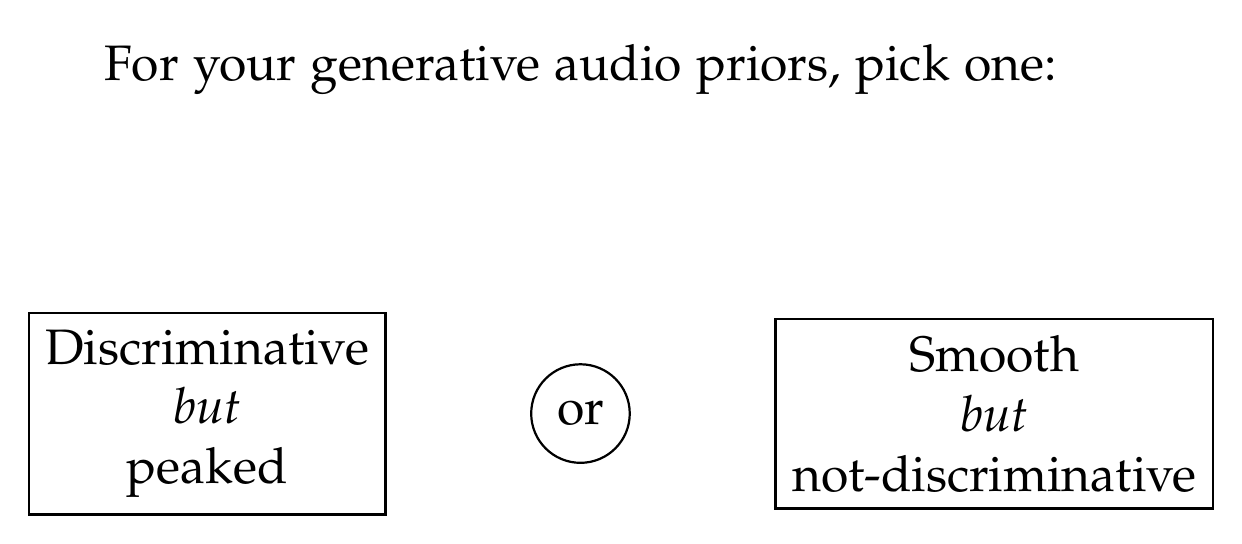
\begin{tikzpicture}[thick,scale=1.8, every node/.style={transform shape}]
            \node[align=center] (pickone) {For your generative audio priors, pick one:};
            \node[draw,circle,below=50pt of pickone] (or) {or};
            \node[draw,rectangle,left=of or,align=center] (discrpeak) {Discriminative\\\textit{but}\\peaked};
            \node[draw,rectangle,right=of or,align=center] (smoothndiscr) {Smooth\\\textit{but}\\not-discriminative};
        \end{tikzpicture}
    }
\end{document}